\newif\ifshowsolutions
\showsolutionstrue
\documentclass{article}
\usepackage{listings}
\usepackage{amsmath}
%\usepackage{subfigure}
% \usepackage{subfig}
\usepackage{amsthm}
\usepackage{amsmath}
\usepackage{amssymb}
\usepackage{graphicx}
\usepackage{mdwlist}
\usepackage[colorlinks=true]{hyperref}
\usepackage{geometry}
\usepackage{titlesec}
\geometry{margin=1in}
\geometry{headheight=2in}
\geometry{top=2in}
\usepackage{palatino}
\usepackage{mathrsfs}
\usepackage{fancyhdr}
\usepackage{paralist}
\usepackage{todonotes}
\setlength{\marginparwidth}{2.15cm}
\usepackage{tikz}
\usetikzlibrary{positioning,shapes,backgrounds}
\usepackage{float} % Place figures where you ACTUALLY want it
\usepackage{comment} % a hack to toggle sections
\usepackage{ifthen}
\usepackage{mdframed}
\usepackage{verbatim}
\usepackage[strings]{underscore}
\usepackage{listings}
\usepackage{bbm}

\usepackage{subcaption}
\usepackage{color}
\rhead{}
\lhead{}

\renewcommand{\baselinestretch}{1.15}

% Shortcuts for commonly used operators
\newcommand{\E}{\mathbb{E}}
\newcommand{\Var}{\operatorname{Var}}
\newcommand{\Cov}{\operatorname{Cov}}
\newcommand{\Bias}{\operatorname{Bias}}
\DeclareMathOperator{\argmin}{arg\,min}
\DeclareMathOperator{\argmax}{arg\,max}

% do not number subsection and below
\setcounter{secnumdepth}{1}

% custom format subsection
\titleformat*{\subsection}{\large\bfseries}

% set up the \question shortcut
\newcounter{question}[section]
\newenvironment{question}[1][]
  {\refstepcounter{question}\par\addvspace{1em}\textbf{Question~\Alph{question}\!
    \ifthenelse{\equal{#1}{}}{}{ [#1 points]}: }}
    {\par\vspace{\baselineskip}}

\newcounter{subquestion}[question]
\newenvironment{subquestion}[1][]
  {\refstepcounter{subquestion}\par\medskip\textbf{\roman{subquestion}.\!
    \ifthenelse{\equal{#1}{}}{}{ [#1 points]:}} }
  {\par\addvspace{\baselineskip}}

\titlespacing\section{0pt}{12pt plus 2pt minus 2pt}{0pt plus 2pt minus 2pt}
\titlespacing\subsection{0pt}{12pt plus 4pt minus 2pt}{0pt plus 2pt minus 2pt}
\titlespacing\subsubsection{0pt}{12pt plus 4pt minus 2pt}{0pt plus 2pt minus 2pt}


\newenvironment{hint}[1][]
  {\begin{em}\textbf{Hint: }}{\end{em}}

\ifshowsolutions
  \newenvironment{solution}[1][]
    {\par\medskip \begin{mdframed}\textbf{Solution~\Alph{question}#1:} \begin{em}}
    {\end{em}\medskip\end{mdframed}\medskip}
  \newenvironment{subsolution}[1][]
    {\par\medskip \begin{mdframed}\textbf{Solution~\Alph{question}#1.\roman{subquestion}:} \begin{em}}
    {\end{em}\medskip\end{mdframed}\medskip}
\else
  \excludecomment{solution}
  \excludecomment{subsolution}
\fi

\newcommand{\boldline}[1]{\underline{\textbf{#1}}}

\chead{%
  {\vbox{%
      \vspace{2mm}
      \large
      Machine Learning \& Data Mining \hfill
      Caltech CS/CNS/EE 155 \hfill \\[1pt]
      Miniproject 2\hfill
      Submitted Feb $26^{\text{th}}$, 2018 \\
    }
  }
}

\begin{document}
\pagestyle{fancy}

\section{Introduction}
\medskip
\begin{itemize}

    \item \boldline{Group members} \\
    Zhewei Chen, Milad Taghavi, Yan Qi Huan
    
    \item \boldline{Team name} \\
    Team MagicMarijuanaForest
    
    \item \boldline{Code repository} \\
    \url{https://github.com/miladtaghavi/Miniproject2}
\end{itemize}

\section{Basic Visualizations}

\begin{figure}[H]
		\centering
		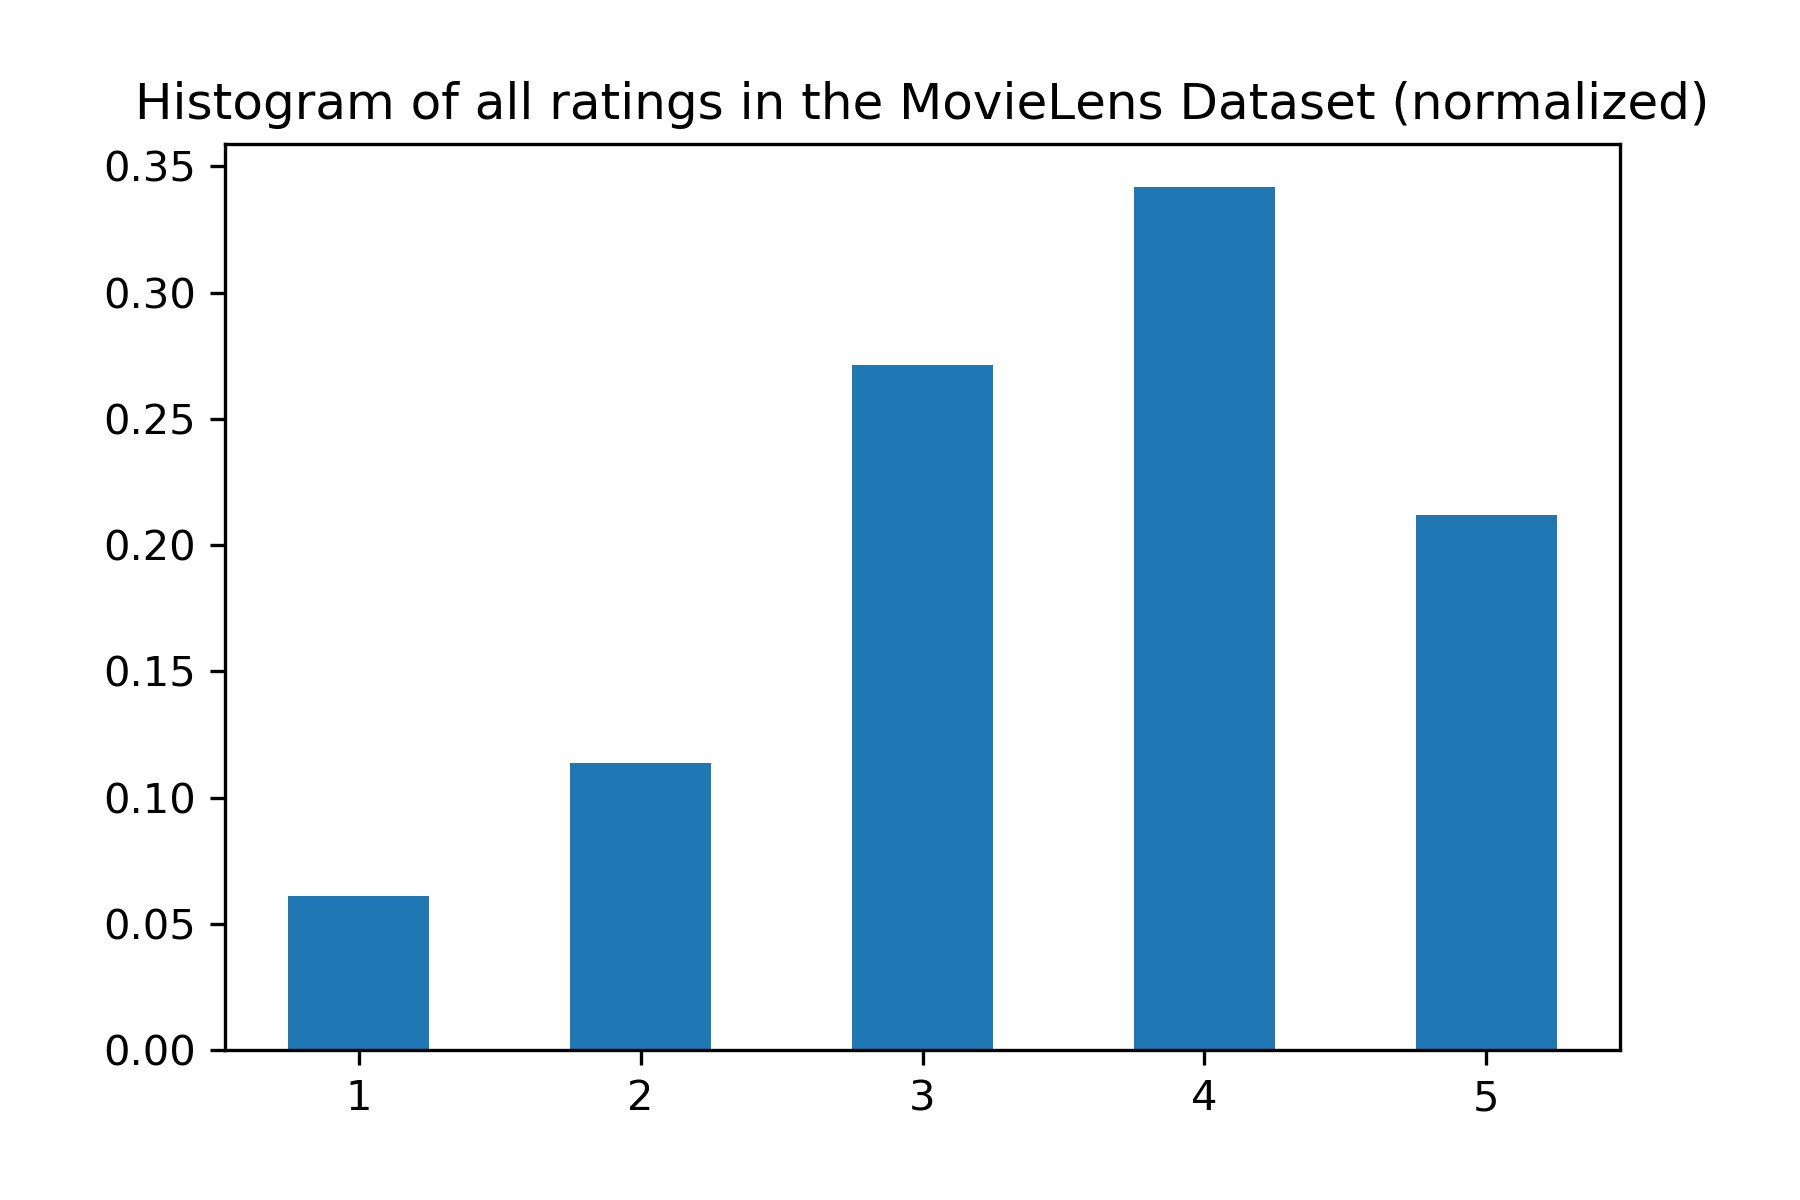
\includegraphics[width=0.5\textwidth]{Fig4-1.png}
		\caption{All ratings in the MovieLens Dateset. We plot the number of ratings with a particular score as a normalized histogram.}
\end{figure}
	
When we plot the distribution of movie ratings over all movies, we see that a majority of ratings are 3 and 4. The mean score over all reviews is 3.53. On average, there are more positive reviews than negative reviews, which is unexpected. This indicates there is a small positive bias in how people rate movies. If movies ratings were unbiased, we should see 3 as the average movie rating over all movies.

\begin{figure}[H]
	\centering
	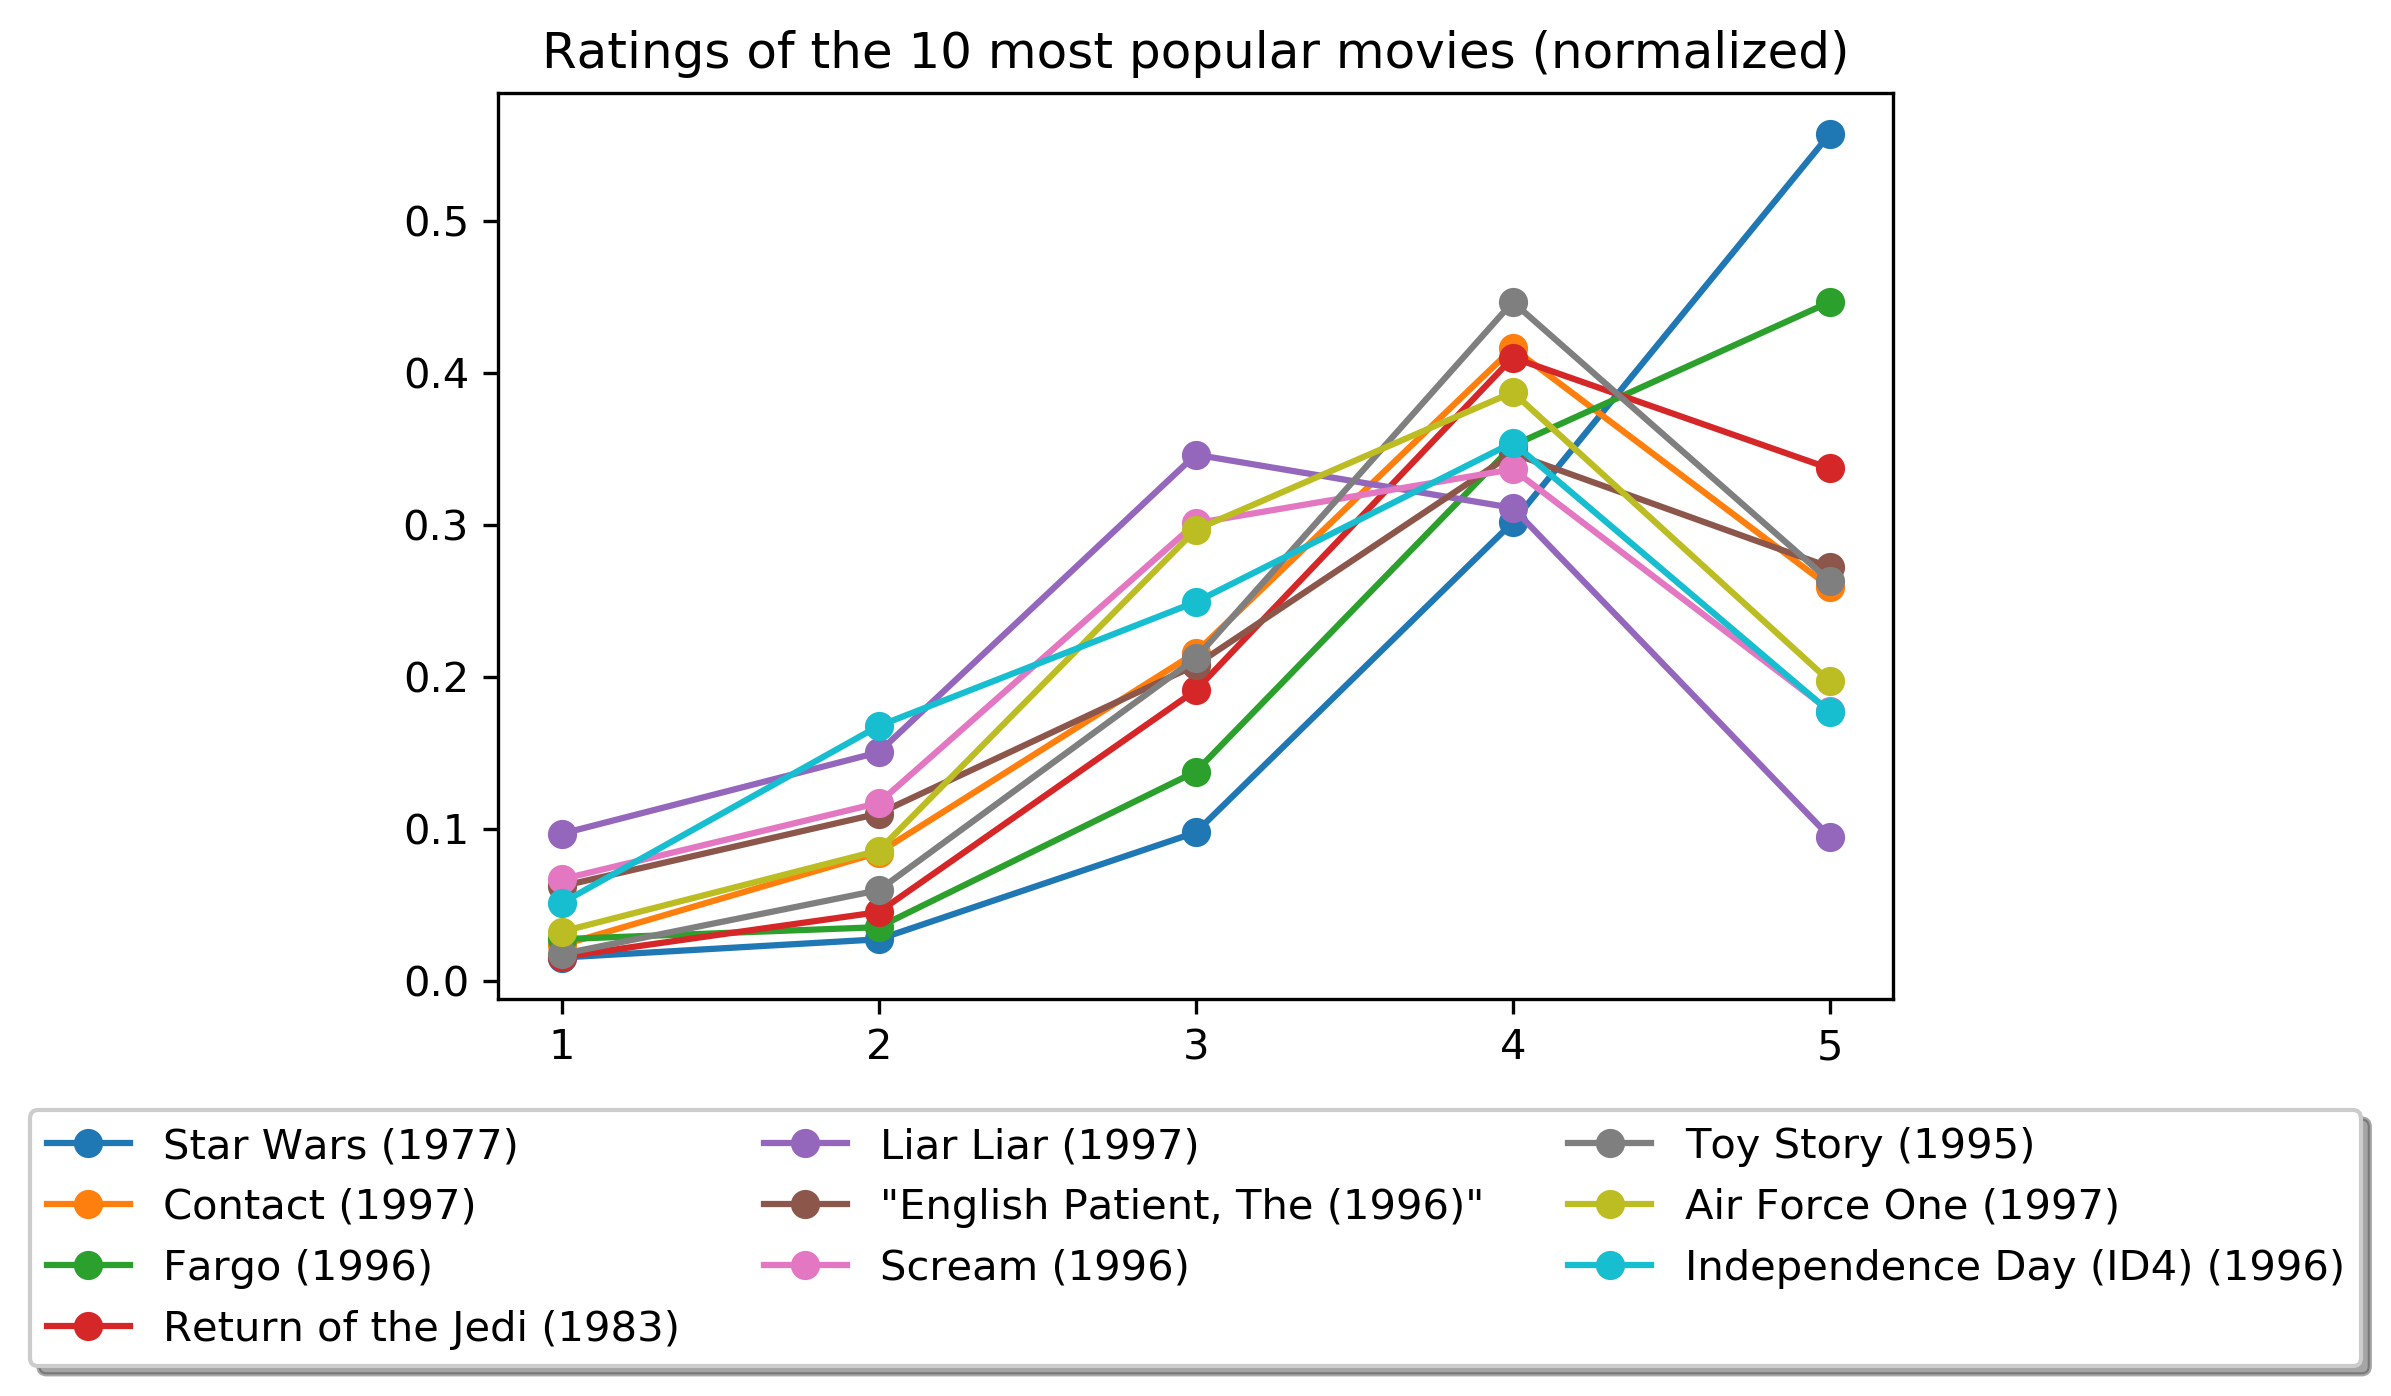
\includegraphics[width=0.8\textwidth]{Fig4-2.png}
	\caption{All ratings of the top 10 most popular movies. We plot the normalized review counts for each of the 10 movies against the score of each review.}
\end{figure}

When we plot the distribution of ratings from the top 10 most popular movies (movies with the most ratings), we see that each movie has its own distribution of ratings, but the overall trend is the same. Popular movies generally get higher ratings, but not everyone is a fan of popular movies. This in fact follows the overall trend over all reviews as plotted above. Of course, there is still a spread of mean scores within these movies, such as Star Wars (mean: 4.36, peaks at score 5) as well as Liar Liar (mean: 3.16, peaks at score 3).

\begin{figure}[H]
	\centering
	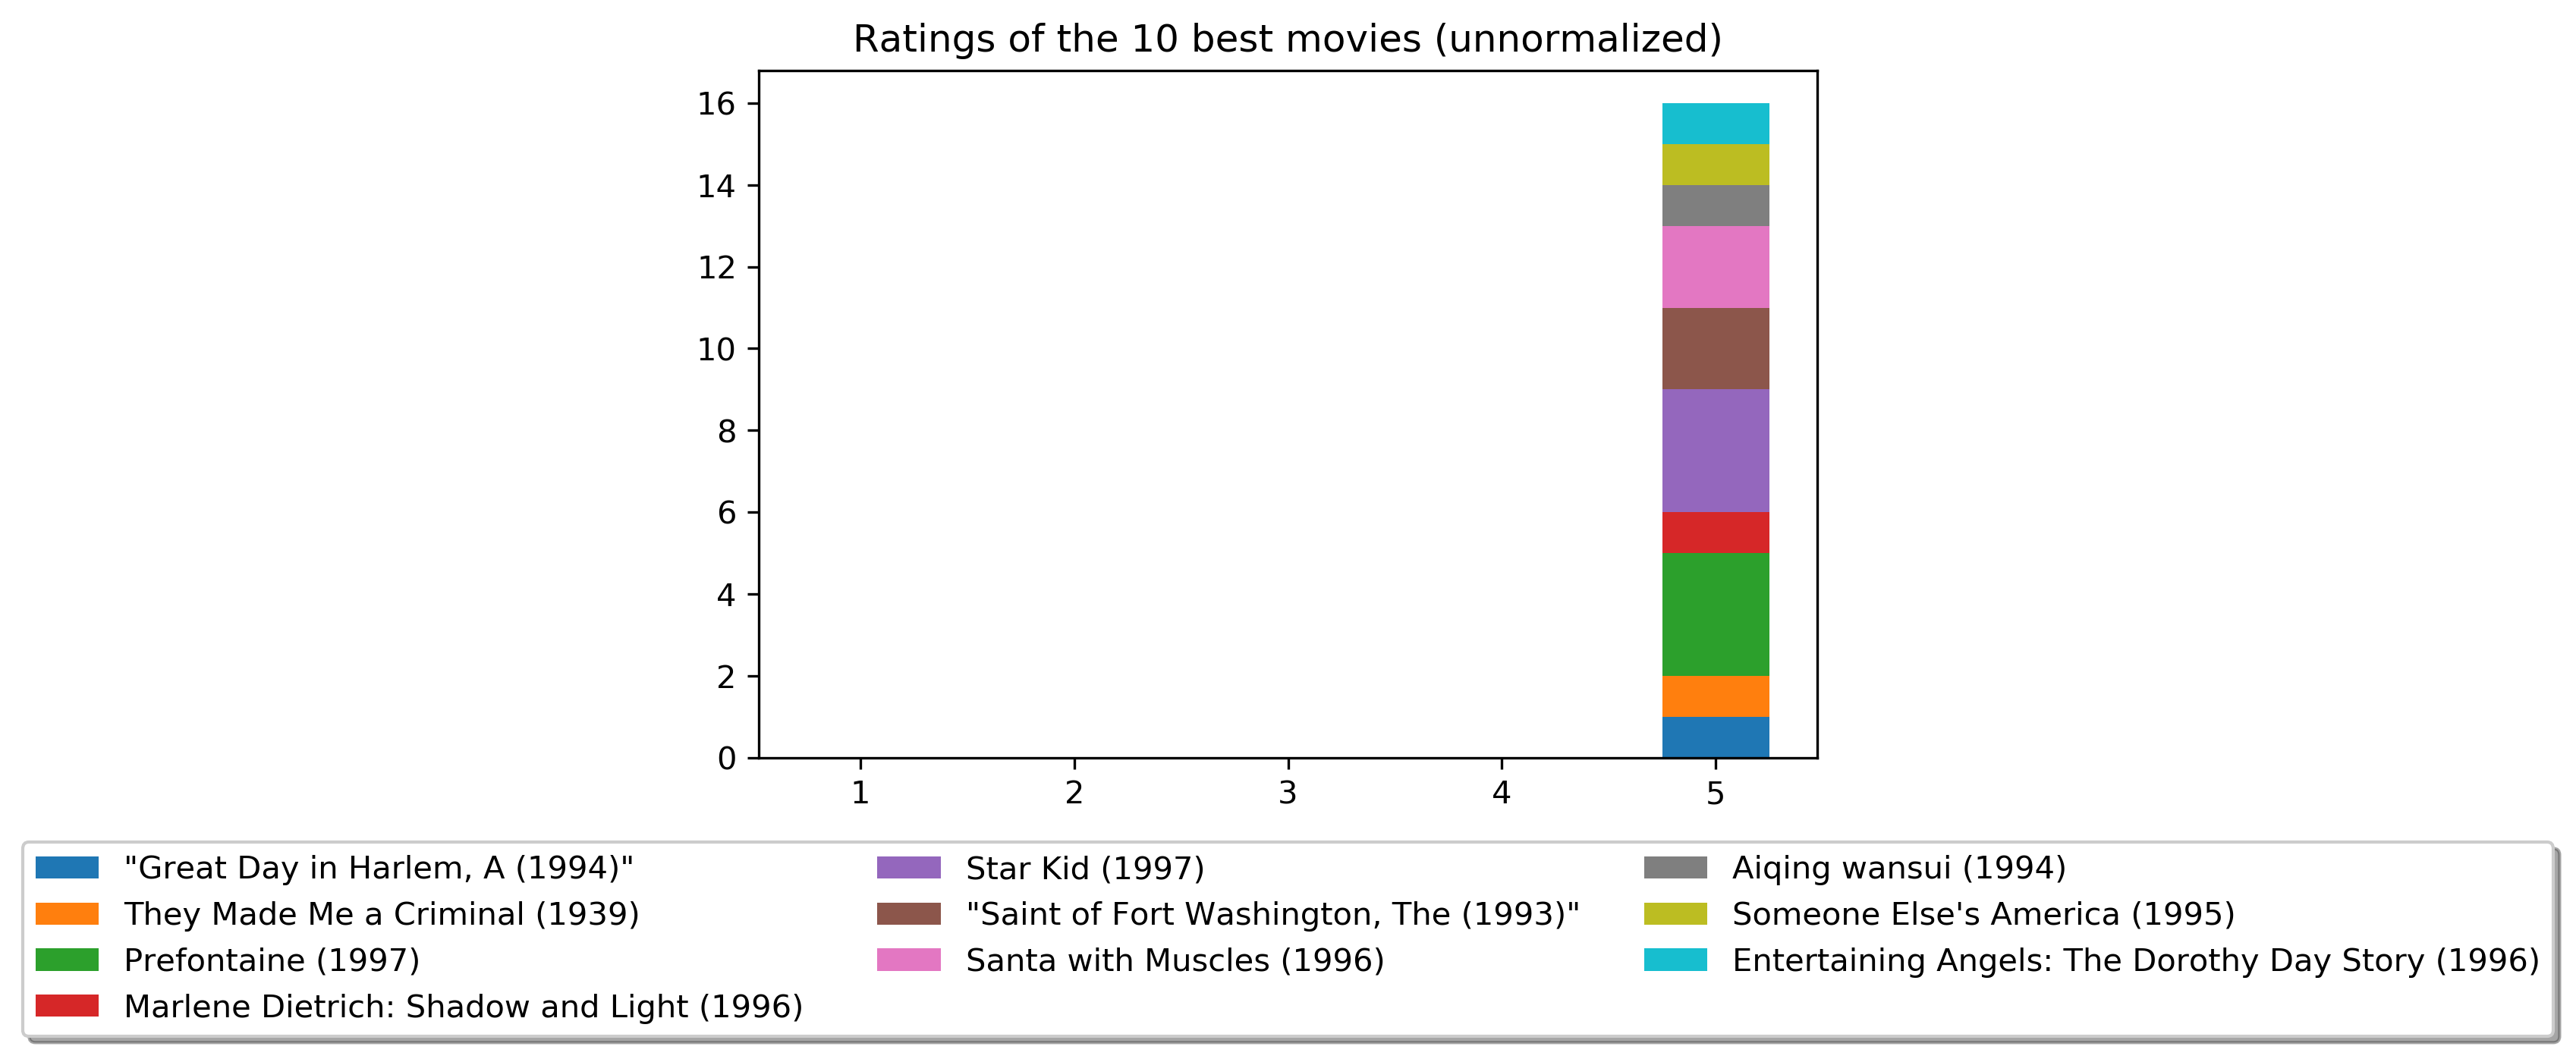
\includegraphics[width=0.8\textwidth]{Fig4-3.png}
	\caption{All ratings of the movies with the top average scores. We use an unnormalized histogram in this case since each movie only has reviews that give it a score of 5. Note that all these movies have less than 5 reviews.}
\end{figure}

When we plotting the distribution of ratings for the top 10 best movies (movies with the highest average ratings), we see that all these movies that have an average score of exactly 5, but have received less than 5 reviews each (this plot was left unnormalized to illustrate this point). These movies are likely under reviewed and the scores given may be biased by certain eclectic movie watchers.

\begin{figure}[H]
	\centering
	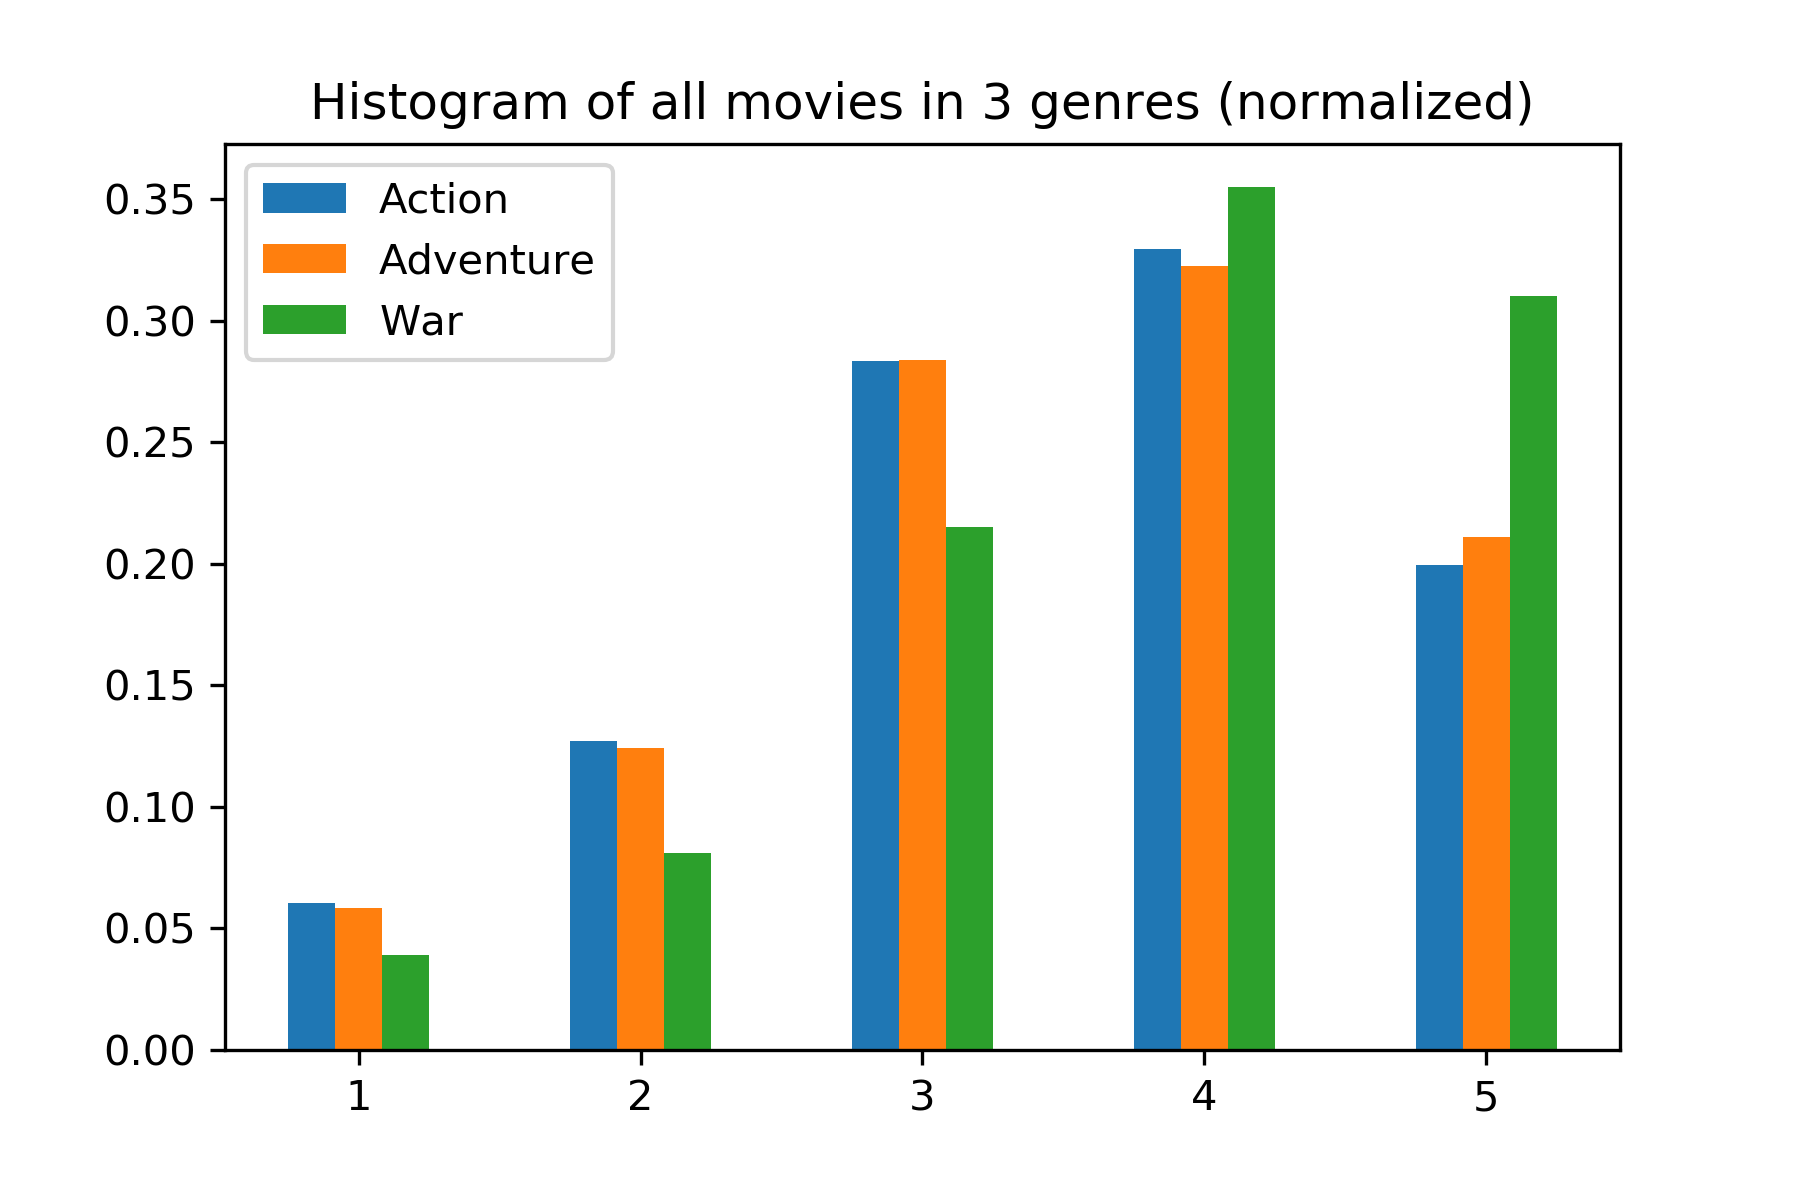
\includegraphics[width=0.5\textwidth]{Fig4-4-4.png}
	\caption{Normalized histogram of scores for movies from the genres Action, Adventure and War.}
\end{figure}

Next, we plot all ratings from 3 genres of our choice. We chose action, adventure and war because they are similar movie genres and should have similar rating distributions. These three genres do have similar rating distributions. The rating distributions also do not differ much from the general trend of all movies. Our selected genres already provide a rough representation of the entire dataset. However, while action and adventure are very similar, war appears to have a much larger skew towards higher scores, as can be seen from its average rating of 3.82 compared to 3.48 and 3.50 for action and adventure respectively.

\section{Matrix Factorization Methods}

\textbf{The 3 Matrix Factorization Methods Used}
\begin{enumerate}
    \item The code from Homework 5, which used a normal matrix factorization method.
    
    \item The code from Homework 5 but with bias terms that represent the average bias in ratings specific to each user and movie.

    \item The surprise package that provided several matrix factorization algorithms, each with tunable parameters.

\end{enumerate}

\textbf{How do each of these methods work? How do they differ?} \newline
    
Method 1 was already introduced in class. Each user and movie were represented as vector of $k$ latent variables which can interact with each other to produce the output score. $m$ users are represented in a $k\times m$ matrix $U$, and all $n$ movies as a $k\times n$ matrix $V$ such that our prediction of each user's rating is simply given by $U^T V$. SGD is used to find the optimal latent matrices which minimize the mean squared error between prediction and actual value. Regularization $\lambda$ on the $L_2$ norm of $U$ and $V$ was used to encourage sparsity in the optimal solution and reduce overfitting. \newline

Method 2 improves upon method 1 $U^T V$ predictions by adding a separate vector $a_i$ and $b_j$ for the $i$-th user and the $j$-th movie. The final output is $Y_{ij}-\mu = u_i^Tv_j + a_i + b_j$. The bias terms account for the tendency of each user to vote higher or lower relative to other users and for each movie to be voted higher or lower than others on average because of hype or external factors. This modification should make the model more accurate as it helps normalize the latent vectors across users and movies. \newline

Method 3 uses the surprise package, an off-the-shelf implementation of various algorithms, including the basic matrix factorization (called SVD) with and without bias (i.e methods 1 and 2 above), non-negative matrix factorization (NMF) with and without bias, as well as another method called SVD++ which takes into account another vector that takes into account \textit{whether} or not a user has rated a particular movie but ignores the actual score of that rating. Unlike the homework implementation, the stopping condition for these algorithms can only be set via the number of epochs of SGD and there is no early stopping condition based on the relative decrease in the loss function. Additionally, there is also the option to individually tweak the regularization parameter for the user vectors and bias as well as the movie vectors and bias separately, but we chose to use a single parameter for simplicity. \newline

\textbf{How did they perform in comparison to one another on the test set?} \newline

Hyperparameter optimization was performed on the regularization parameter $\lambda$ while $\kappa=20$ was fixed. In addition to optimization on $\lambda$, in the surprise package, we also played with the SVD method with and without bias to see how latent vector outputs differed.

\begin{figure}[H]
	\centering
	\begin{subfigure}[t]{0.3\textwidth}
		\centering
		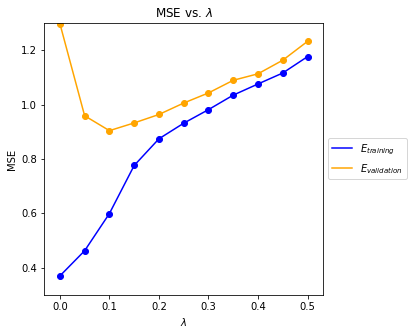
\includegraphics[width=\textwidth]{MatrixFactor_hw}
		\caption{Method 1: Matrix factorization using HW 5 code.}
	\end{subfigure}%
	\begin{subfigure}[t]{0.3\textwidth}
		\centering
		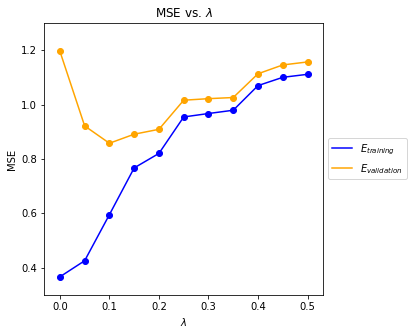
\includegraphics[width=\textwidth]{MatrixFactorBias_hw}
		\caption{Method 2: Same as method 1 but including bias terms}
	\end{subfigure}
	\begin{subfigure}[t]{0.3\textwidth}
		\centering
		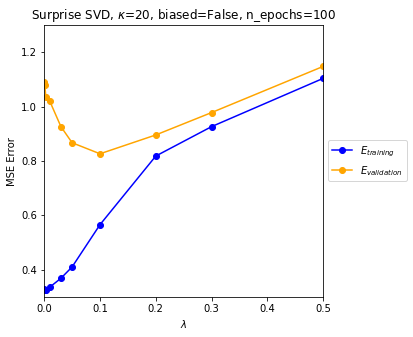
\includegraphics[width=\textwidth]{SVDNoBias_RegErr}
		\caption{Method 3: Using the $SVD()$ method in the surprise package}
	\end{subfigure}
	\caption{Learning curve of matrix factorization as a function of regularization parameter $\lambda$ for the 3 methods. The optimal parameter in all 3 methods were found to be 0.1.}
\end{figure}

The figure above shows the learning curves for the 3 methods. For the surprise package, we only showed the results for the SVD method without bias, with 20 latent factors and 100 SGD epochs. The optimal regularization weight $\lambda$ for all three methods was $\lambda=0.1$.

The mean squared test error of all three methods was about 0.9. Adding the bias term improved test accuracy slightly, which was expected. Method 3 gave approximately the same result as Method 1, but ran much much faster, which was an advantage when we wanted to play with other features in the package. \newline

\begin{figure}[H]
	\centering
	\begin{subfigure}[t]{0.3\textwidth}
		\centering
		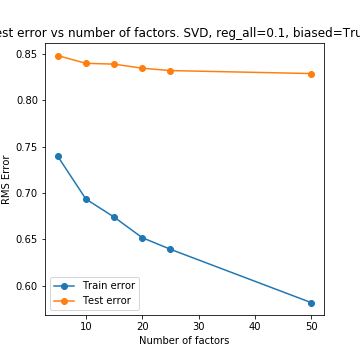
\includegraphics[width=\textwidth]{Surprise_EpB}
		\caption{Method 3 with Bias}
	\end{subfigure}
	\begin{subfigure}[t]{0.3\textwidth}
		\centering
		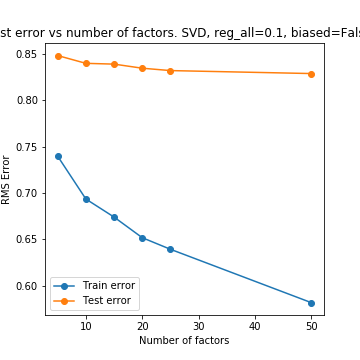
\includegraphics[width=\textwidth]{Surprise_EpNoB}
		\caption{Method 3 without Bias}
	\end{subfigure}
\end{figure}

For method 3, we also looked at varying the number of latent factors $\kappa$ and fixing $\lambda=0.1$. Increasing the number of latent factors marginally improved test accuracy, so we stayed with $\kappa=20$. There was not much difference in performance between matrix factorization with and without bias.

\begin{figure}[H]
	\centering
	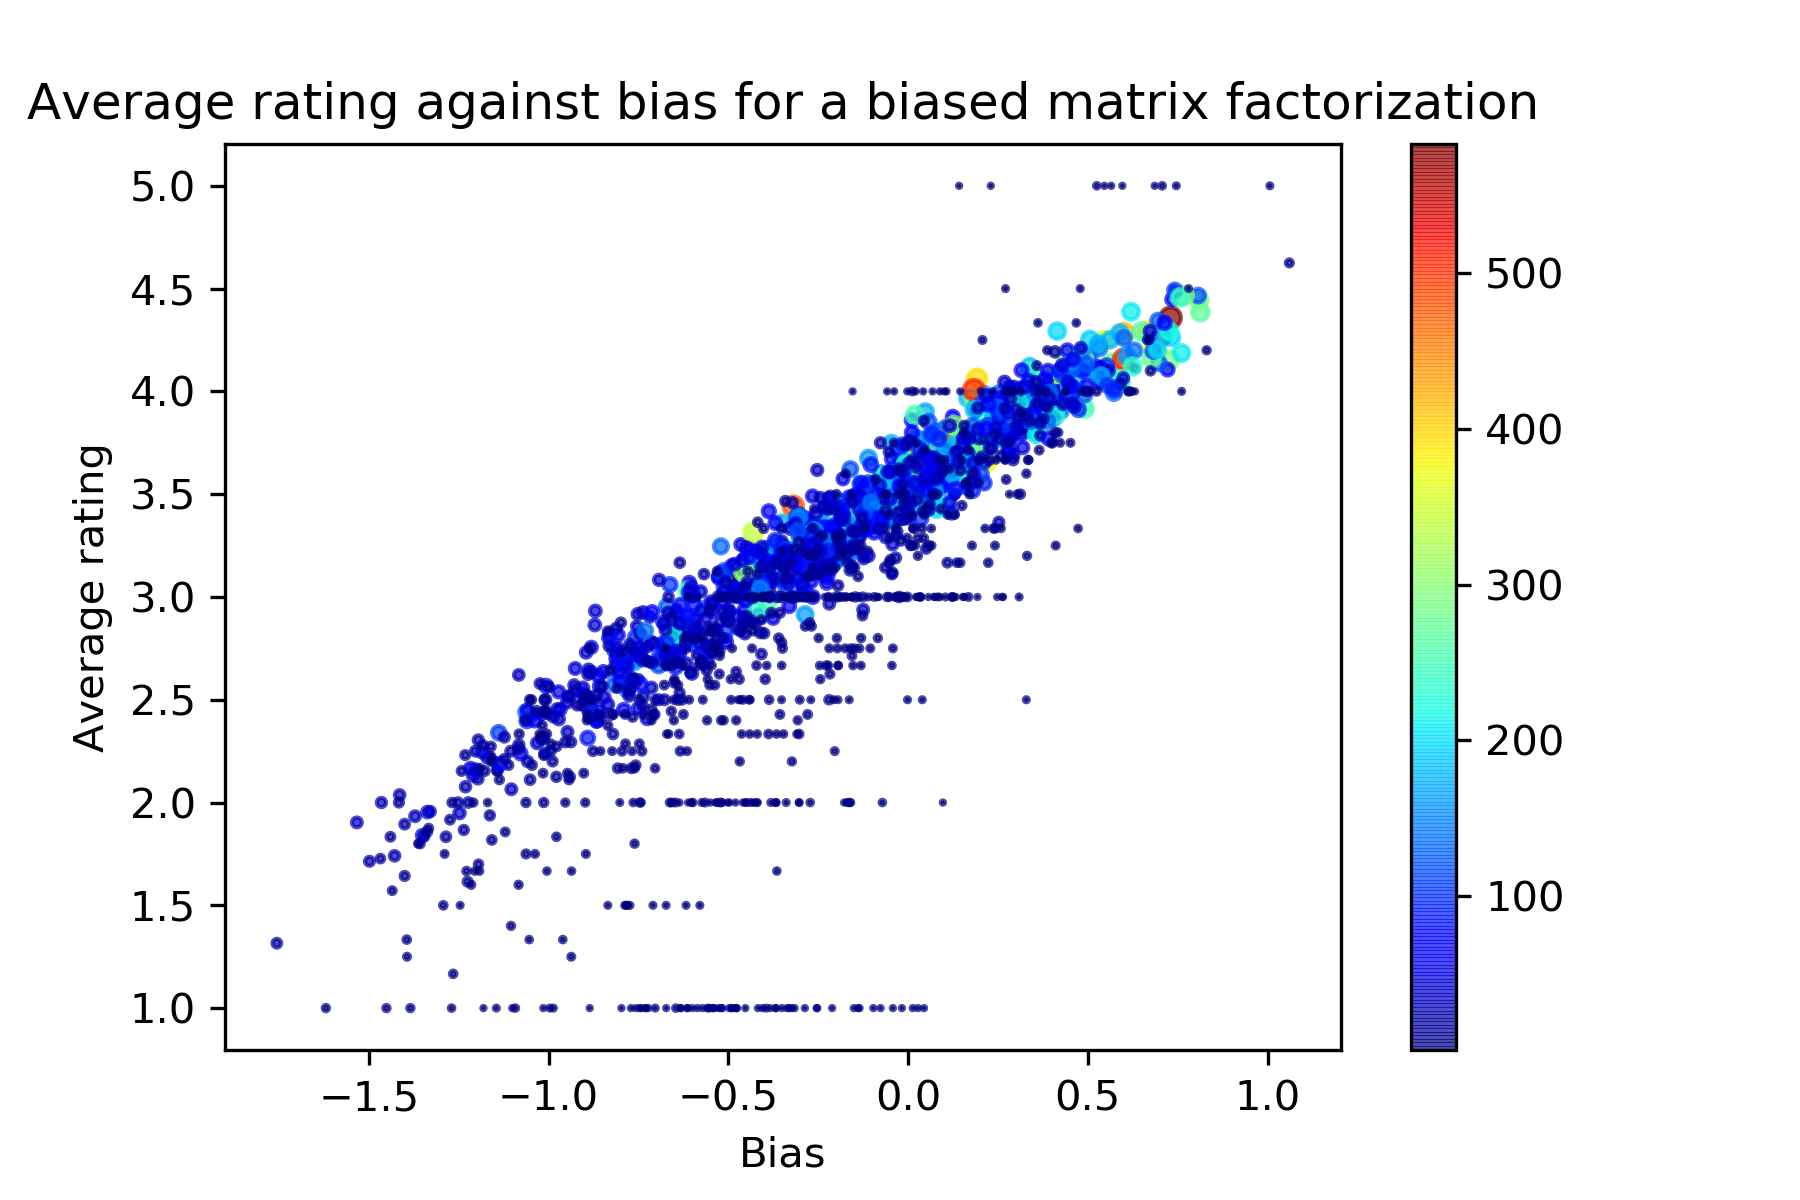
\includegraphics[width=0.7\textwidth]{RatingVsBias.png}
	\caption{Method 2 data. Size and color of circles represent number of reviews given for a specific movie.}
\end{figure}

Another preliminary visualization we did was to plot the average bias term for each movie against that movie's average rating. The color and size of each point represent the number of ratings given to the particular movie. As expected, the bias term was able to capture the average rating given by all users for a particular movie. However, its unclear what information the resulting latent movie vectors still contain. The latent movie vectors between biased and unbiased factorization are different from each other. \newline

\section{Matrix Factorization Visualizations}

From the matrix factorization algorithms in the previous section, we obtained 2 matrices $U$ and $V$ that are suited for analysis. As suggested in the set, we applied SVD to the $V$ matrix of movie vectors and projected $V$ onto a 2-dimensional space based on the first 2 singular vectors. This gave us a 2-dimensional space to visualize our data. \newline

Here the visualizations for $V$ vector found from method 3 both with and without bias is provided only. Method 3 without bias is generally equivalent to Method 1. Method 3 with bias is generally equivalent to Method 2. \newline

A quick glance at the SVD coeffients of $\Sigma$ shows that the first principle explain the most variation in the movie vector. The second and successive components show only marginally more information. The first two components together explain about 30 percent of total variability, meaning PCA might not be a good representation of latent vectors in high dimensional space.

$Sigma = [64.52, 17.23, 13.01, 12.06, 11.46, \dots 8.89]$ from matrix factorization without Bias

\begin{figure}[H]
	\centering
	\begin{subfigure}[t]{0.4\textwidth}
		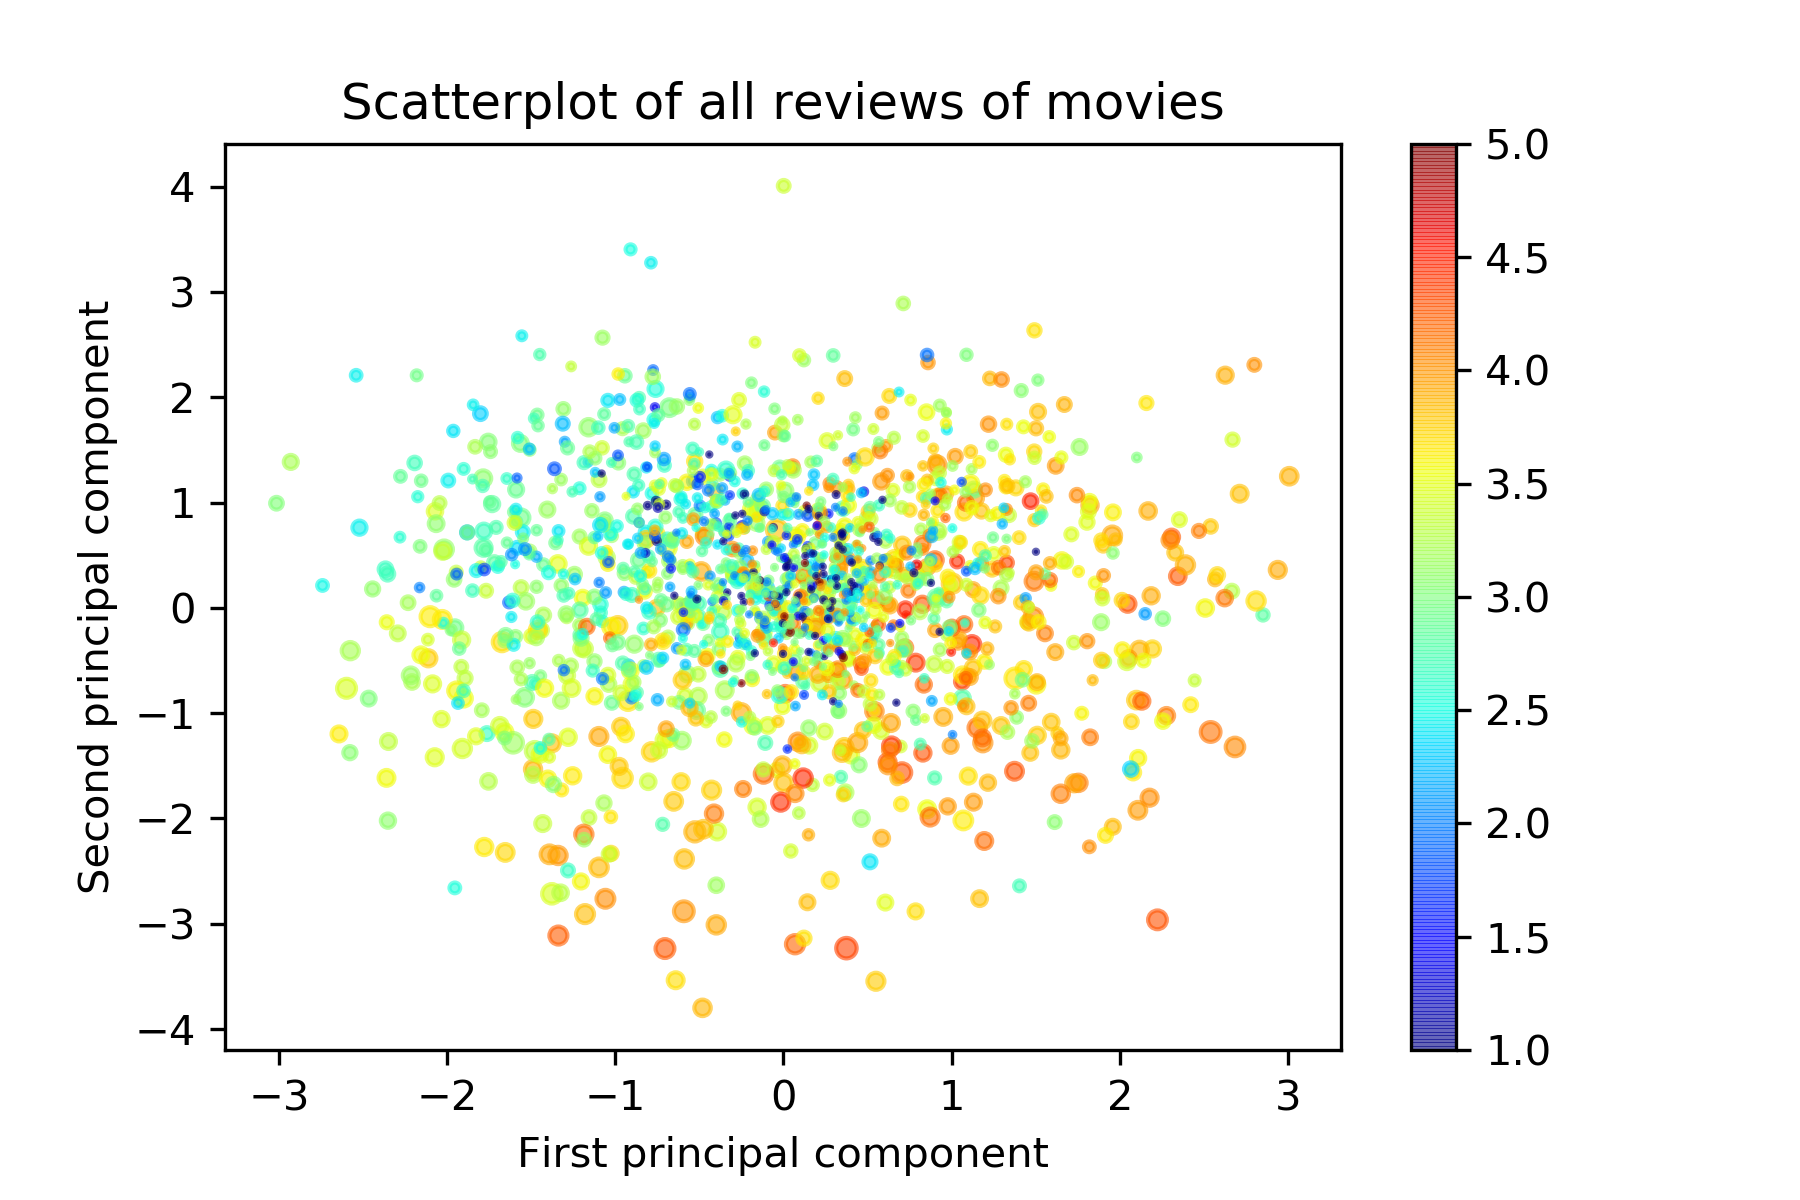
\includegraphics[width=\textwidth]{ScoresBias.png}
		\caption{Method 3 with Bias}
	\end{subfigure}
	\begin{subfigure}[t]{0.4\textwidth}
		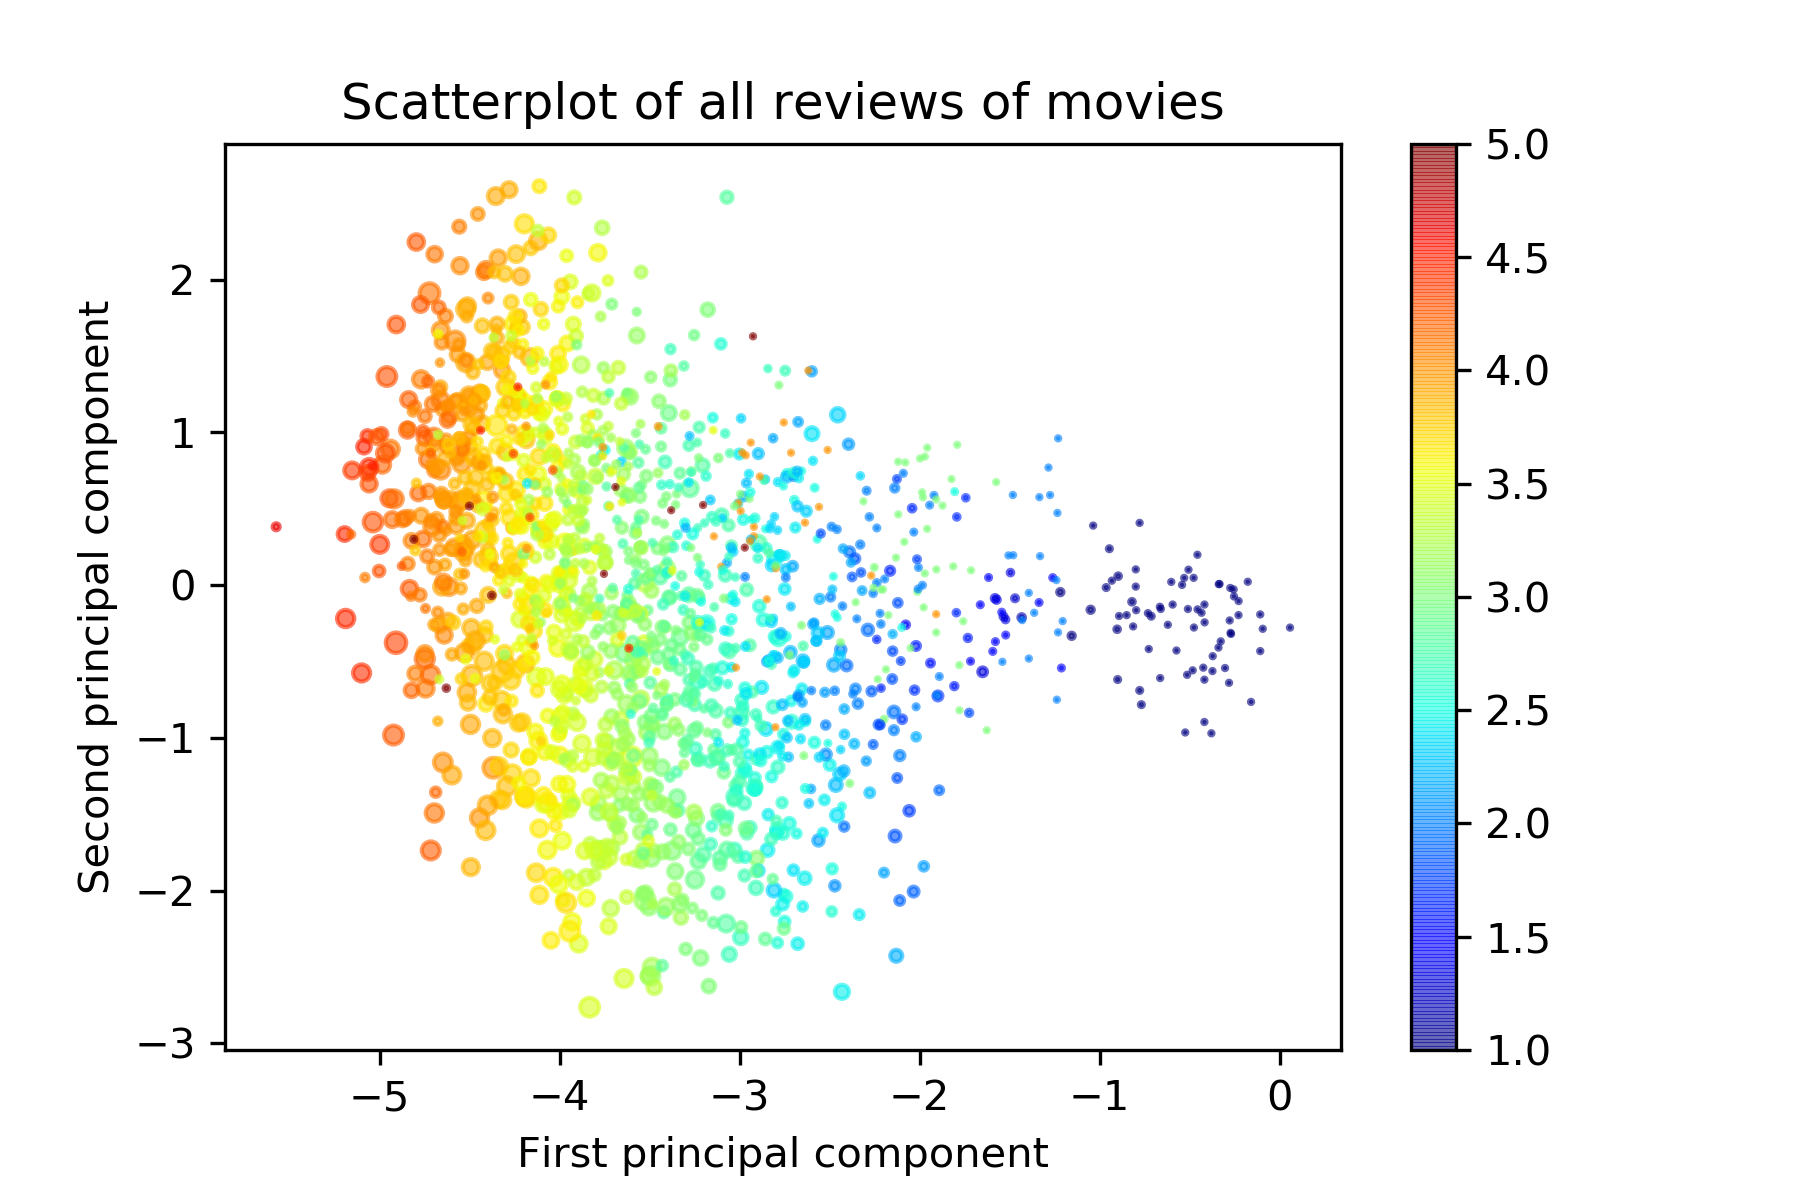
\includegraphics[width=\textwidth]{ScoresRaw.png}
		\caption{Method 3 without Bias}
	\end{subfigure}
	\caption{Average Rating Score (color bar) are strongly determined by the first principal component. The size of the data point corresponds to the number of reviews given to that movie.}
\end{figure}

For latent vectors calculated with bias, we see that lower scoring movies are generally in the center of plot while higher scoring movies are farther from the origin. The minor differences in how the latent vectors were calculated significantly influences the way the latent vectors are visualized. We are still uncertain what information is contained in the latent movie vectors. However, for the unbiased case, we know the first component strongly determines average movie rating score. Here, we can also see an island of movies which are under-reviewed and rated poorly. \newline

Some of these points are likely outliers, so we decided to filter out the movies with less than 30 reviews. As a result of this filtering, the island of movie vectors disappeared and data points are more strongly categorized by the first principal component.

\begin{figure}[H]
	\centering
	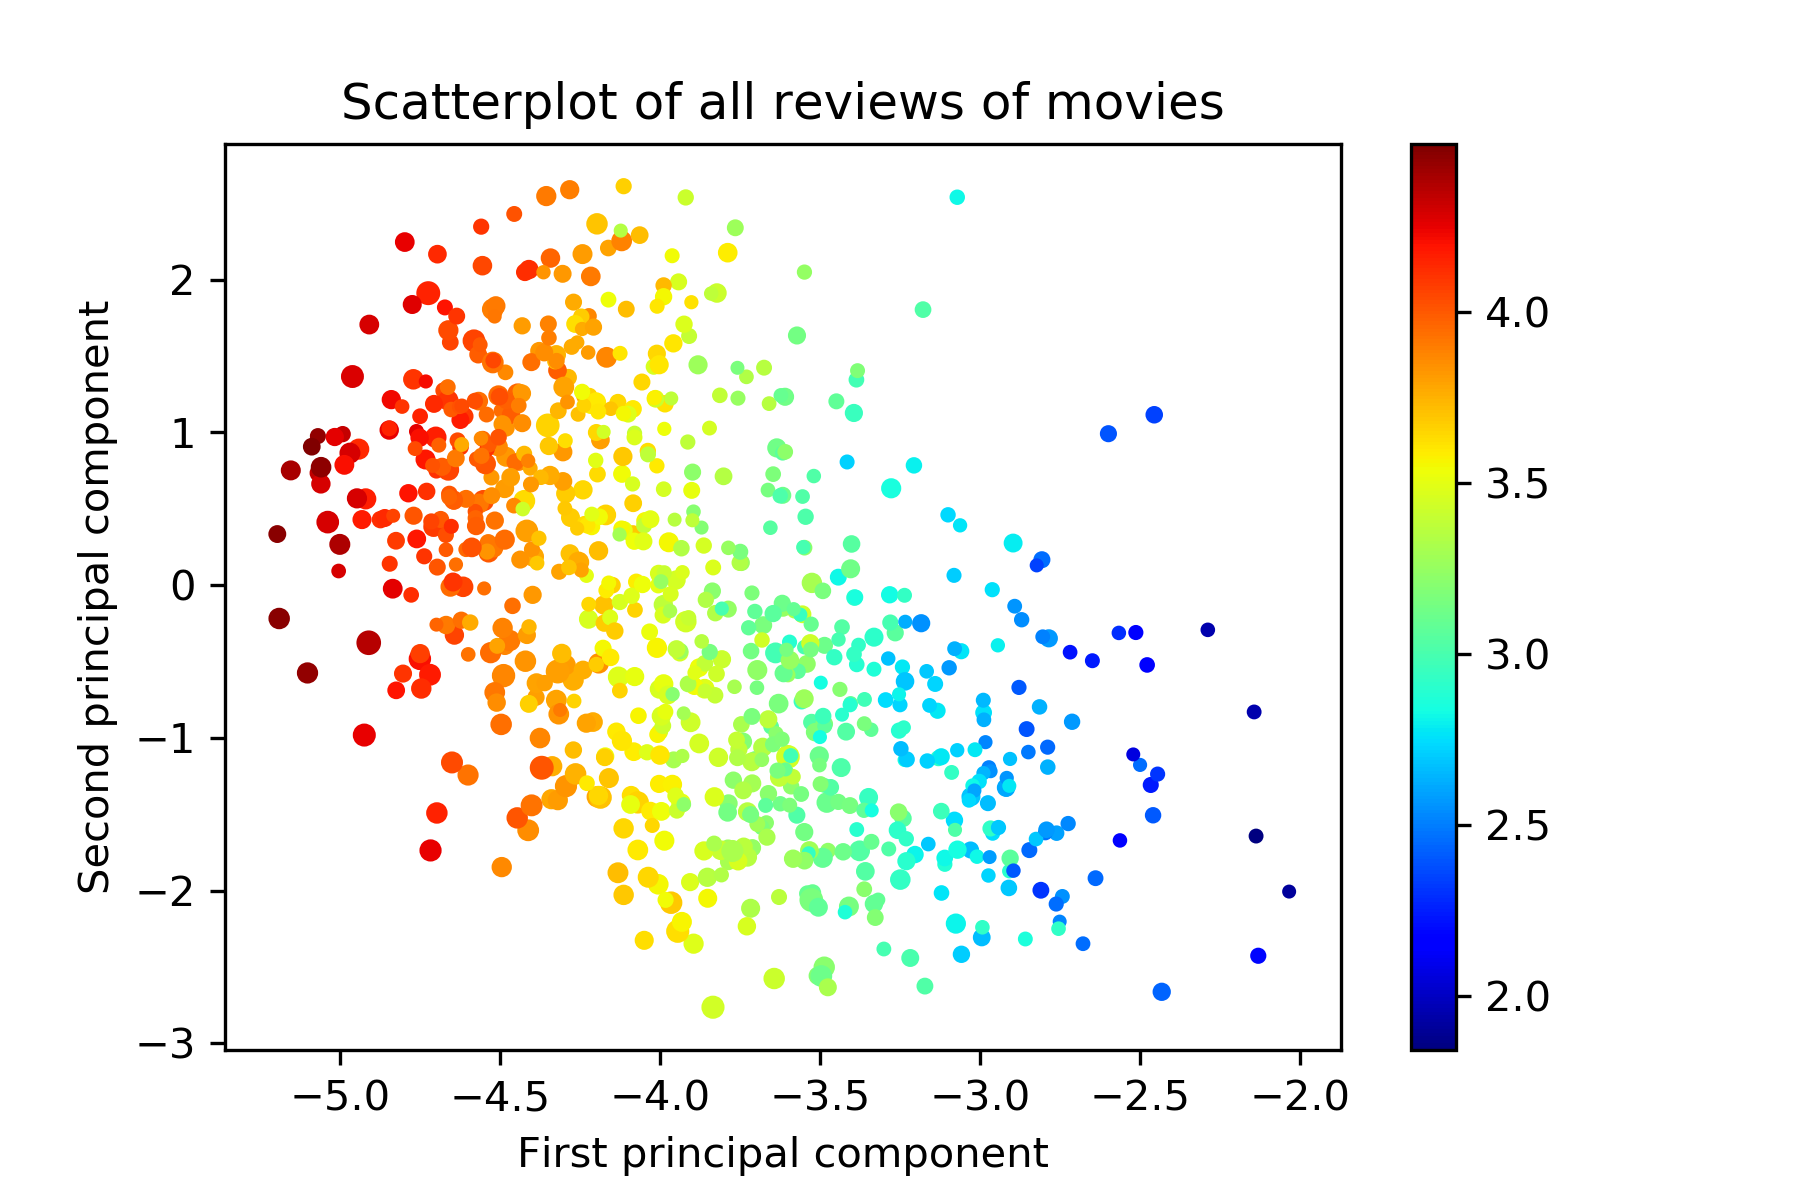
\includegraphics[width=0.7\textwidth]{Scores30Raw.png}
	\caption{Method 3 without Bias. Movies with less than 30 reviews are filtered out from the previous plot. As a result of this filtering, the island of movie vectors disappears. The isolated red dots (highly rated movies, but few reviews) also disappear.}
\end{figure}


\begin{figure}[H]
	\centering
	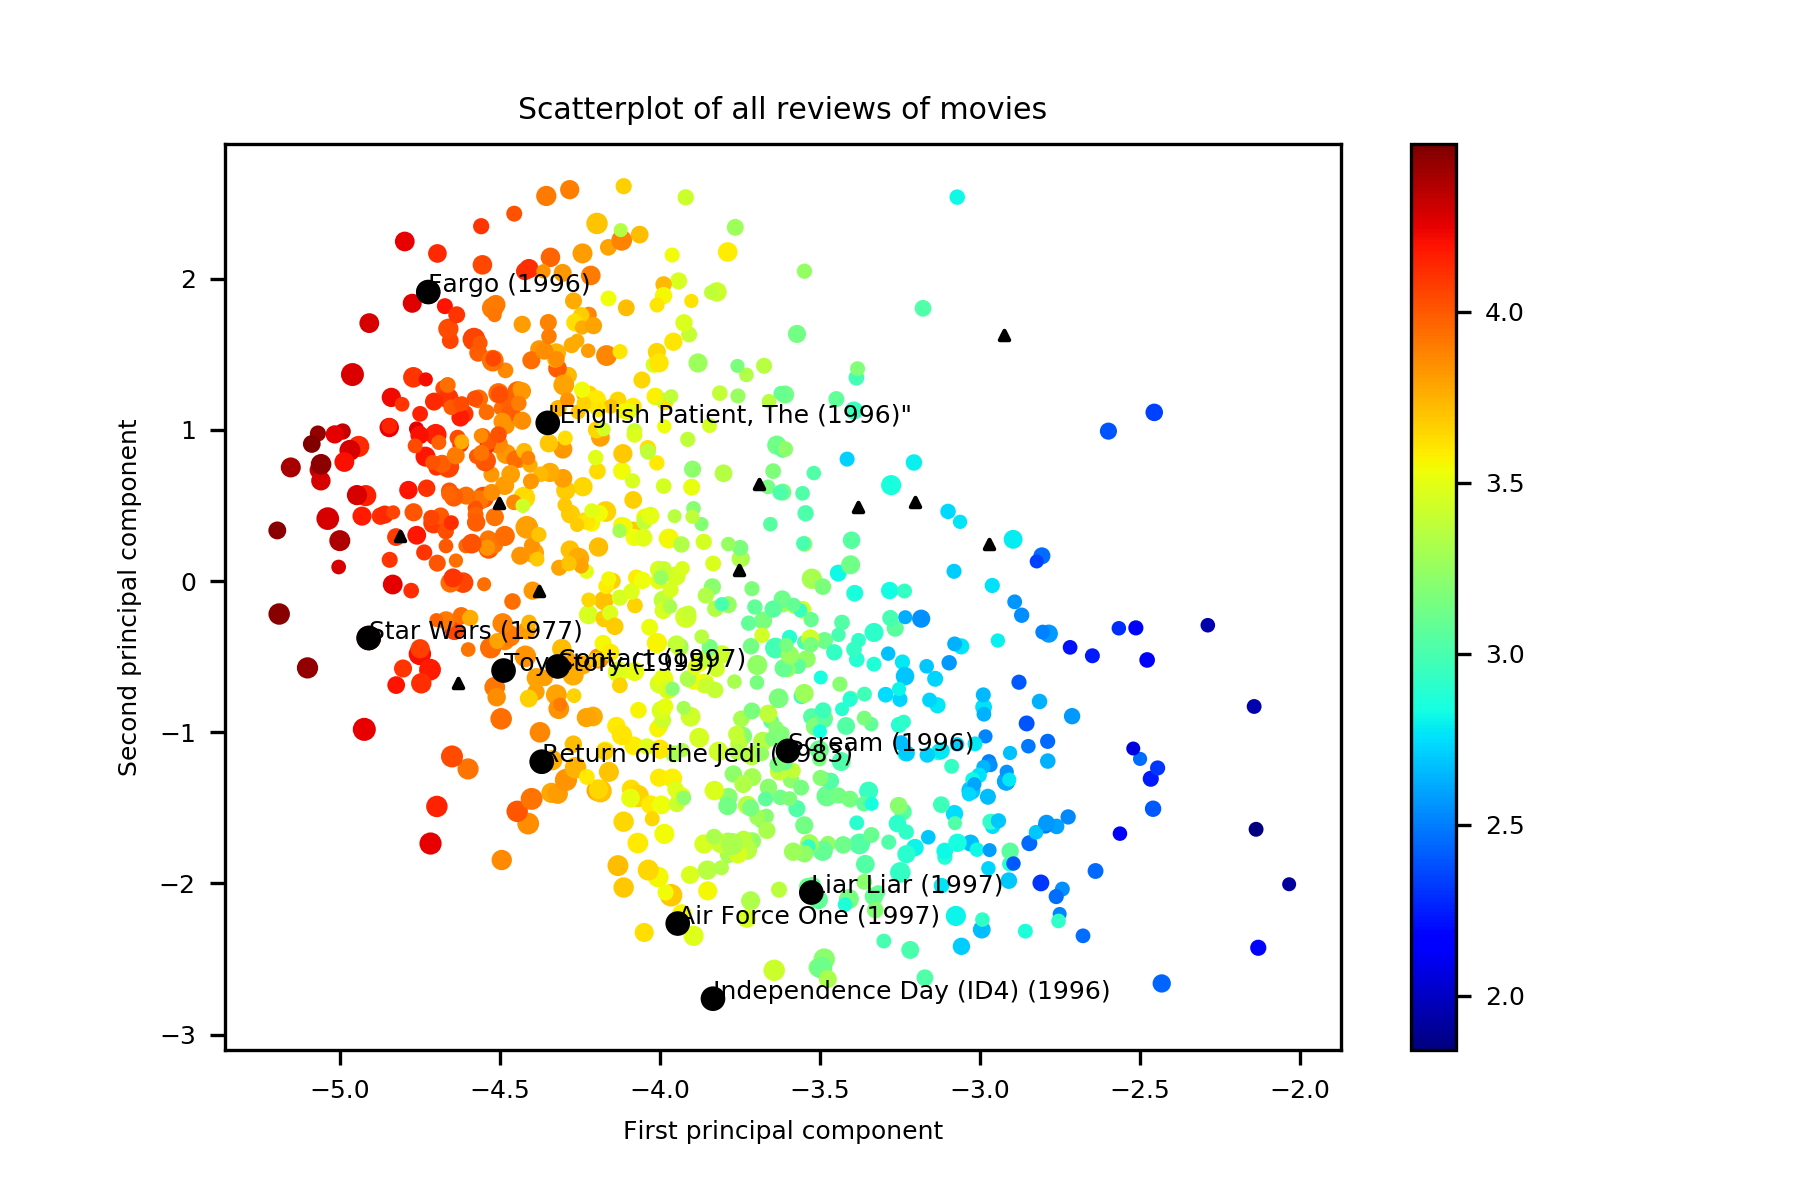
\includegraphics[width=1.0\textwidth]{Scores30Labelled.png}
	\caption{Here the top ten most rated movies marked in black circles. The top ten most highly rated movies are in black triangles. The size of the markers correspond to the number of ratings. Here we also excluded movies which have less than 30 reviews to filter out potentially noisy outlier movie ratings.}
\end{figure}

The above figure shows the top ten most rated and highly rated movies in black circles and triangles respectively. Here we keep the filter applied in the previous part. As we can see the top ten most rated movies would be perfectly categorized by with a definitive range of the first principal component. The 10 most highly rated movies; however, could not be strongly categorized by the first two components.

\begin{figure}[H]
	\centering
	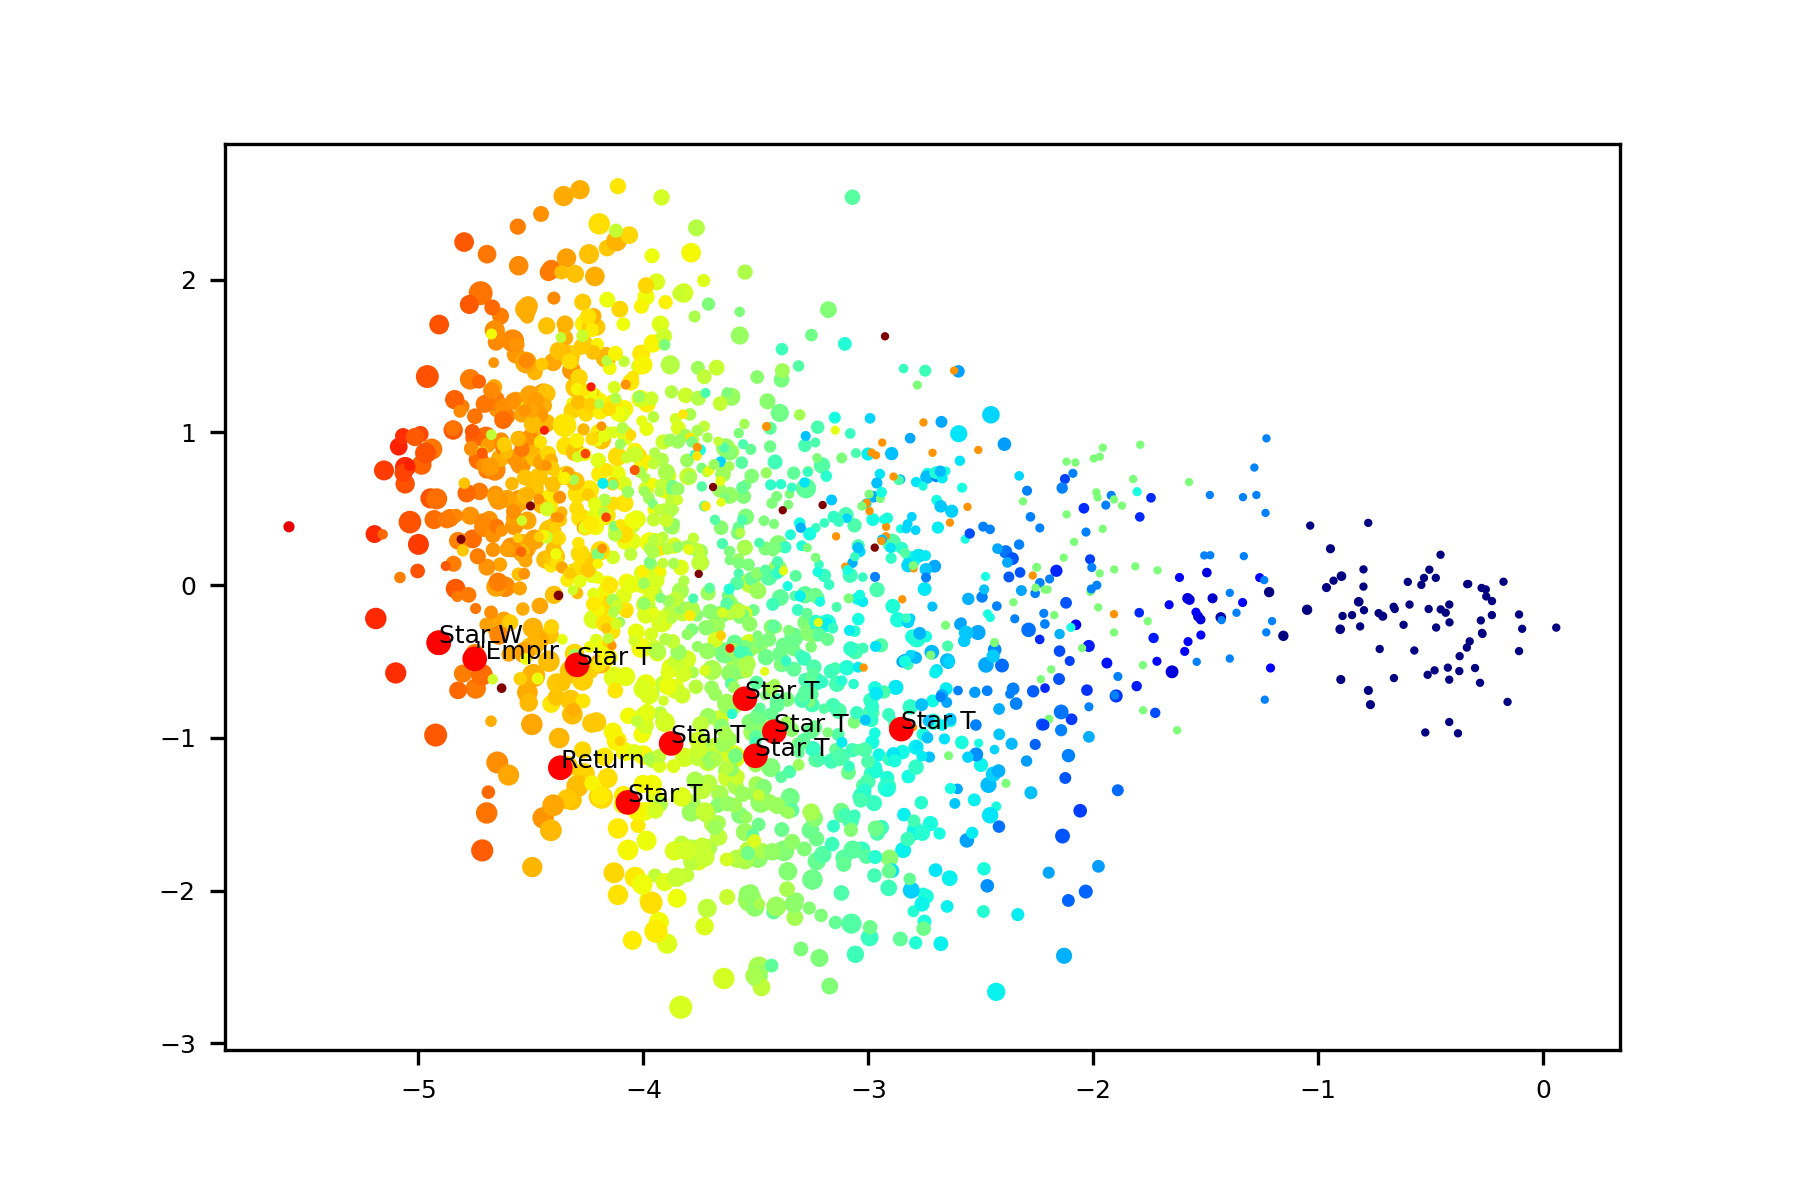
\includegraphics[width=1.0\textwidth]{Star.png}
	\caption{10 movies of our choice - 3 were from Star Wars and the remaining 7 were from Star Trek (Names are shortened due to space constraints). We see that these generally tend to congregate in the bottom left quadrant of the plot, indicating the expected similarity between these movies. There is also a weak separation between the Star Wars movies and the Star Trek movies.}
\end{figure}

In the above figure, we chose the 10 movies of our choice from star wars and star trek movies. These movies are all located in limited range of the first and second principal component. since these movies share a same spectrum of audience with the same interests. 

\begin{figure}[H]
	\centering
	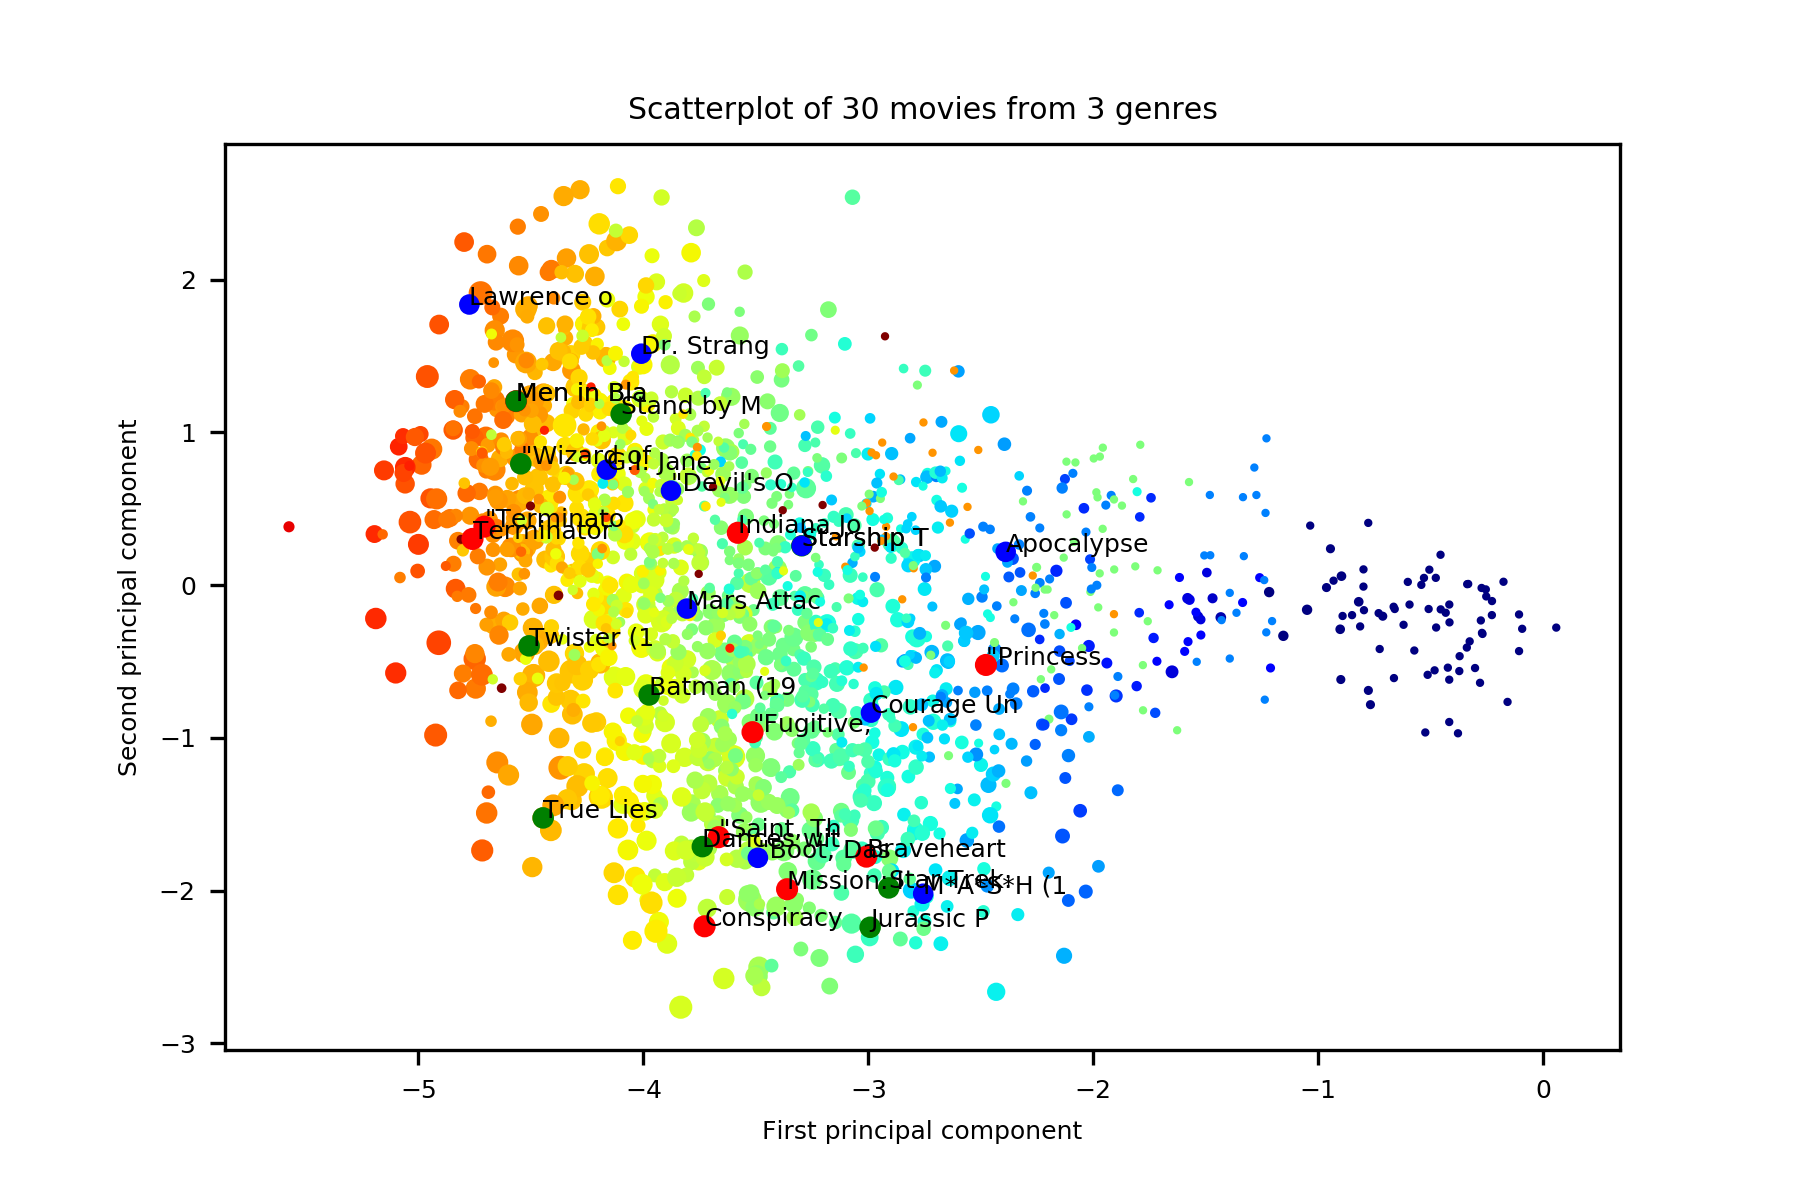
\includegraphics[width=1.0\textwidth]{3Genres.png}
	\caption{Scatter plot of 10 movies from 3 genres: Action (Red), Adventure (Green), and War (Blue). Movie names are shortened due to space constraints. The movies chosen were the 10-20th most rated for each genre (we omitted the top 10 to avoid using the same points as Figure 11,12).}
\end{figure}

In the figure above, we have plotted the 10 movies from each genres of Action (Red), Adventure (Green), and War (Blue). To avoid using the same data point as in Figure 11 and 12, the 10-20th most rated movies from each genre is selected. As we can see, since there are less rating in the 10-20th movies, we see more variation as compared to Figure 11. Also, although the movie genres chosen to have the most overlap in the audience and their interest, the data point are still located in a small range of variations in the first two principal components.


\begin{figure}[H]
	\centering
	\begin{subfigure}[t]{0.4\textwidth}
		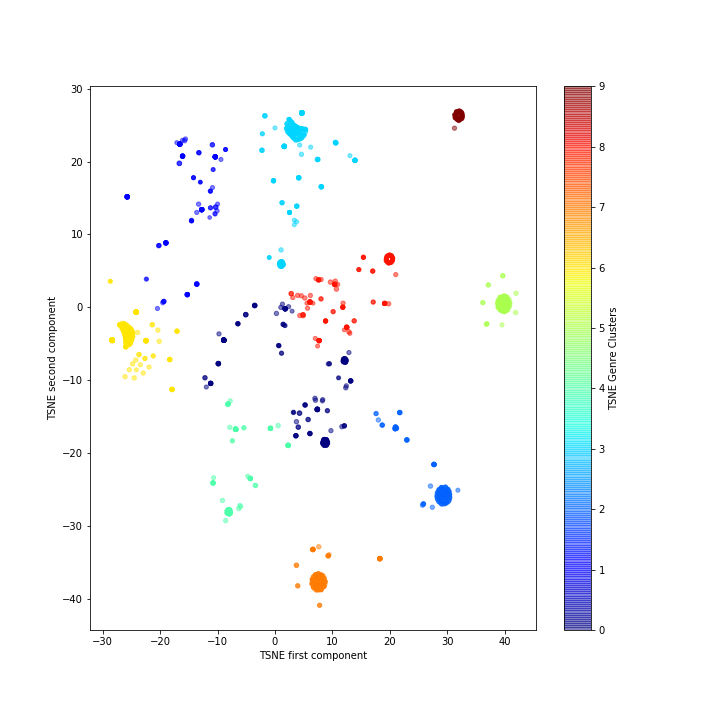
\includegraphics[width=\textwidth]{TSNEcluster.png}
		\caption{Mutually exclusive genre clusters obtained via t-SNE.}
	\end{subfigure}
	\begin{subfigure}[t]{0.4\textwidth}
		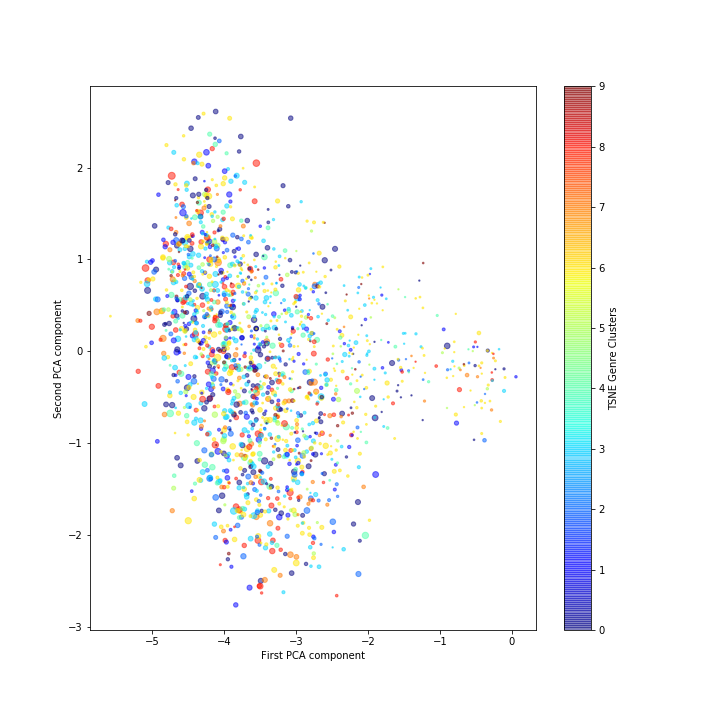
\includegraphics[width=\textwidth]{TSNE_PCA_cluster.png}
		\caption{Mapping of genre clusters to PCA of latent movie vectors}
	\end{subfigure}
	\caption{Colors represent classes of mutually exclusive genres obtained via k-means. The size of the data point corresponds to the number of reviews given to that movie.}
\end{figure}

In the above figures, we wish to see if the latent movie vectors actually mapped to specific genre classes. For this task we need to classify movies into mutually exclusive genre classes. We used t-SNE (t-distributed Stochastic Neighbor Embedding) to compress the high-dimensional genre vectors into a 2-dimensional representation. K-means clustering (with $k=10$ clusters) was applied to the 2-dimensional t-SNE data. \newline

We see that the latent movie vectors are not good separators of the genre classes. We hypothesize that this is due to the fact that there is a distribution of both good and bad reviews within each genre cluster and that there are users who like multiple genres. Thus, it is likely hard to magically map genre information back to the movie vectors in these sorts of models.

\end{document}
